\documentclass[a4paper,11pt,oneside]{article}
\usepackage{tabularx}
\usepackage{fancybox}
\usepackage{amsmath}
\usepackage[top=1.5in,bottom=1in,right=1in,left=1in,headheight=65pt]{geometry}
\usepackage{graphicx}
\usepackage{fancyhdr}

%Gummi|065|=)
\begin{document}
\pagestyle{fancy}

\fancyhead[L]{Stevens UPEPC\\12 April 2014}
\fancyhead[C]{{\LARGE\textbf{Time Out}}}
\fancyhead[R]{
\includegraphics[height=32pt]{../stevenslogo.eps}\ \ \ 
\includegraphics[height=32pt]{../upelogo.png}}


\section{Problem Statement}

Steven's digital clock seems to be malfunctioning. When he checked the time at various
points throughout the day, he noticed that some of the LCD segments are not working.
\\\\
He recalls having seen the displays:
\begin{center}
\begin{tabularx}{7in}{X X X X}

\includegraphics[height=40pt]{./assets/testclock_1.eps}&

\includegraphics[height=40pt]{./assets/testclock_2.eps}&

\includegraphics[height=40pt]{./assets/testclock_3.eps}&
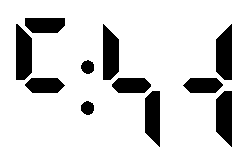
\includegraphics[height=40pt]{./assets/clock_4.eps}
\end{tabularx}
\end{center}
Based on what he has seen, can Steven determine the current time, shown by last clock display,
with 100\% certainty?

\section{Input}
The first line of input contains a single integer $\boldsymbol{P}$,
$(\boldsymbol{1} \le \boldsymbol{P} \le \boldsymbol{1000})$, which is the
number of data sets that follow. Each data set should be processed identically
and independently.
\\\\
Each data set begins with a single line that contains $\boldsymbol{K}$, the data
set number, followed by $\boldsymbol{N}$,
$(\boldsymbol{1} \le \boldsymbol{N} \le \boldsymbol{10})$ which is the number
of clock displays that will be given. Note that Steven does not
remember the clock displays in order and he may have seen them any time in the past
12 hours. Steven's clock uses a 12-hour format (\texttt{15:00} is not a valid time).
\\\\
The next $\boldsymbol{N}$ lines  contain the clock displays that Steven has seen.
The clock displays are given in the format $(d_1\ d_2\ d_3\ d_4)$ where $d_0$ is
the tens digit of the hour and $d_4$ is the ones digit of the minutes. Being as
the digits in the display may not be consist of full digits, each will be given as
a binary representation of the LCD segments that are active (see below). The last
line of each data set indicates the current clock time that you must determine.

\subsection{Digit Representation}
\begin{tabularx}{\textwidth}{@{}X r@{}}
\parbox[m]{10cm}{Digits are binary-encoded. Being as there are 7 LCD segments that
make up each digit, they will be encoded as an integer value such that the $i$th segment
is active in a display $D$ iff the $i$th least significant bit is set in $D$.
\\\\
For example, the digit ``5'' would be encoded as:
\begin{center}
$\texttt{1110011}_2 = 2^0 + 2^1 + 2^2 + 2^5 + 2^6 = 103_{10}$
\end{center}
} & \parbox[m]{5cm}{
\includegraphics[height=120pt]{./assets/digit_binary.eps}} \\
\end{tabularx}
\\\\\\
The digits 0-9 are displayed as follows with their decimal encodings given below.
\begin{center}
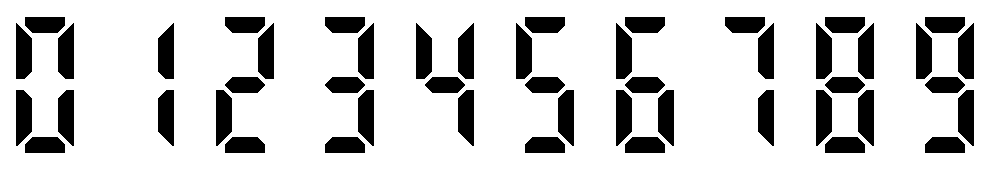
\includegraphics[width=4.9in]{./assets/all_numbers.eps}
\begin{tabularx}{5in}{@{}>{\centering}X >{\centering}X >{\centering}X >{\centering}X >{\centering}X >{\centering}X >{\centering}X >{\centering}X >{\centering}X >{\centering}X@{}}
123 & 72 & 61 & 109 & 78 & 103 & 119 & 73 & 127 & 111
\end{tabularx}
\end{center}

\section{Output}
For each data set there is a single line of output. The single line of output
consists of the data set number $\boldsymbol{K}$, followed by a single space
followed by the real value of the current clock time $\boldsymbol{T}$. The time you output
should be in regular human-readable 12-hour clock format, i.e ``\texttt{11:59}''
or ``\texttt{2:30}''. If it is impossible to determine with 100\% certainty
what the current time is, your program should output a single question mark (\texttt{?}) instead.

\section{Test Data}
\begin{tabularx}{\textwidth}{|X|X|}
	\hline
	Input & Output \\ \hline
	\parbox[t]{5cm}{
	\texttt{3\\
			1 4\\
			8 27 101 28\\
			0 9 35 90\\
			0 14 70 76\\
			0 7 70 76\\
			2 4\\
			8 27 101 28\\
			0 9 35 88\\
			0 14 70 76\\
			0 7 70 76\\
			3 1\\\
			72 61 103 127\\
	}} & \parbox[t]{5cm}{
	\texttt{1 5:43\\
			2 ?\\
			3 12:58\\
	}}\\
	\hline
\end{tabularx}
\begin{center}
\begin{tabularx}{7in}{X X X X}

\includegraphics[height=40pt]{./assets/testclock_1.eps}&

\includegraphics[height=40pt]{./assets/testclock_2.eps}&

\includegraphics[height=40pt]{./assets/testclock_3.eps}&
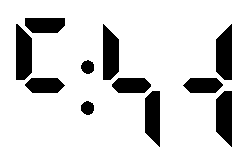
\includegraphics[height=40pt]{./assets/clock_4.eps}
\end{tabularx}
\end{center}
\textbf{Test Case \#1:}\\
You will have to convince yourself that for the first test case, which uses the 4 displays
shown above, the only time that is possible for the last clock display is
\texttt{5:43}. For example, the time cannot be \texttt{5:44} because the top left segment of the
last digit is not lit in that display, but it is lit in the second display.
Therefore it must be working, so for the last digit of the current time to be a ``\texttt{4}'',
this segment would have to be lit.
\\\\
\textbf{Test Case \#2:}\\
In the second test case, this is not the case. The top left segment of the last digit is not lit
in any of the displays that have been seen, so therefore it is possible that the last digit could
be a ``\texttt{3}'', ``\texttt{4}'' or ``\texttt{9}''. Being as there are multiple possibilities,
we cannot say with 100\% certainty, so the output is simply ``\texttt{?}''.
\\\\
\textbf{Test Case \#3:}\\
In the last test case, the only clock display seen reads ``\texttt{12:58}''. Please convince yourself
that there exist no other possible times given this observation.

\end{document}